\section{Burger's Equation}
In this problem you will solve Burgers equation, $u_t+f_x= 0,\ f=\frac{1}{2}u^2,\ x \in [0,4)$, periodic boundaries, with the initial condition shown below.

\begin{figure}[h]
    \centering
    

\tikzset{every picture/.style={line width=0.75pt}} %set default line width to 0.75pt        

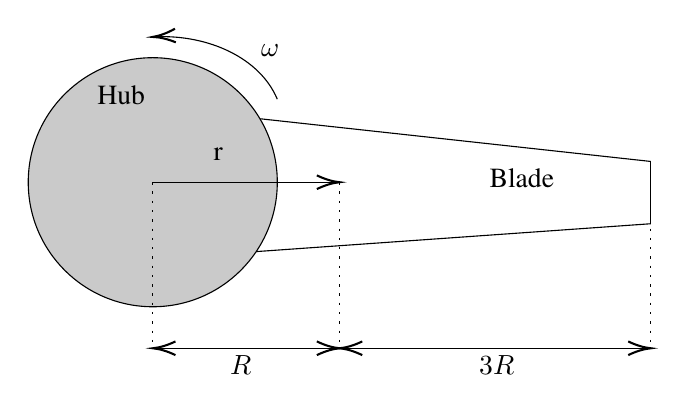
\begin{tikzpicture}[x=0.75pt,y=0.75pt,yscale=-1,xscale=1]
%uncomment if require: \path (0,300); %set diagram left start at 0, and has height of 300

%Shape: Circle [id:dp6244430308199536] 
\draw  [fill={rgb, 255:red, 202; green, 202; blue, 202 }  ,fill opacity=1 ] (220,120) .. controls (220,86.86) and (246.86,60) .. (280,60) .. controls (313.14,60) and (340,86.86) .. (340,120) .. controls (340,153.14) and (313.14,180) .. (280,180) .. controls (246.86,180) and (220,153.14) .. (220,120) -- cycle ;
%Straight Lines [id:da1433381310737285] 
\draw    (520,110) -- (520,140) ;
%Straight Lines [id:da6958270078143212] 
\draw    (520,110) -- (331.79,89.43) ;
%Straight Lines [id:da5982890152434965] 
\draw    (520,140) -- (329.79,153.43) ;
%Straight Lines [id:da7103183675633375] 
\draw    (280,120) -- (368,120) ;
\draw [shift={(370,120)}, rotate = 180] [color={rgb, 255:red, 0; green, 0; blue, 0 }  ][line width=0.75]    (10.93,-3.29) .. controls (6.95,-1.4) and (3.31,-0.3) .. (0,0) .. controls (3.31,0.3) and (6.95,1.4) .. (10.93,3.29)   ;
%Straight Lines [id:da18697245418380692] 
\draw  [dash pattern={on 0.84pt off 2.51pt}]  (280,120) -- (280,200) ;
%Straight Lines [id:da9445115873305969] 
\draw  [dash pattern={on 0.84pt off 2.51pt}]  (370,120) -- (370,200) ;
%Straight Lines [id:da8681269156370801] 
\draw    (282,200) -- (368,200) ;
\draw [shift={(370,200)}, rotate = 180] [color={rgb, 255:red, 0; green, 0; blue, 0 }  ][line width=0.75]    (10.93,-3.29) .. controls (6.95,-1.4) and (3.31,-0.3) .. (0,0) .. controls (3.31,0.3) and (6.95,1.4) .. (10.93,3.29)   ;
\draw [shift={(280,200)}, rotate = 0] [color={rgb, 255:red, 0; green, 0; blue, 0 }  ][line width=0.75]    (10.93,-3.29) .. controls (6.95,-1.4) and (3.31,-0.3) .. (0,0) .. controls (3.31,0.3) and (6.95,1.4) .. (10.93,3.29)   ;
%Straight Lines [id:da9459156094037822] 
\draw    (372,200) -- (518,200) ;
\draw [shift={(520,200)}, rotate = 180] [color={rgb, 255:red, 0; green, 0; blue, 0 }  ][line width=0.75]    (10.93,-3.29) .. controls (6.95,-1.4) and (3.31,-0.3) .. (0,0) .. controls (3.31,0.3) and (6.95,1.4) .. (10.93,3.29)   ;
\draw [shift={(370,200)}, rotate = 0] [color={rgb, 255:red, 0; green, 0; blue, 0 }  ][line width=0.75]    (10.93,-3.29) .. controls (6.95,-1.4) and (3.31,-0.3) .. (0,0) .. controls (3.31,0.3) and (6.95,1.4) .. (10.93,3.29)   ;
%Straight Lines [id:da5900923017563646] 
\draw  [dash pattern={on 0.84pt off 2.51pt}]  (520,120) -- (520,200) ;
%Curve Lines [id:da19047210809641868] 
\draw    (340,80) .. controls (331.57,59.94) and (306.65,48.98) .. (281.9,49.91) ;
\draw [shift={(280,50)}, rotate = 356.45] [color={rgb, 255:red, 0; green, 0; blue, 0 }  ][line width=0.75]    (10.93,-3.29) .. controls (6.95,-1.4) and (3.31,-0.3) .. (0,0) .. controls (3.31,0.3) and (6.95,1.4) .. (10.93,3.29)   ;

% Text Node
\draw (331,52.4) node [anchor=north west][inner sep=0.75pt]    {$\omega $};
% Text Node
\draw (316,202.4) node [anchor=north west][inner sep=0.75pt]    {$R$};
% Text Node
\draw (436,202.4) node [anchor=north west][inner sep=0.75pt]    {$3R$};
% Text Node
\draw (252,72) node [anchor=north west][inner sep=0.75pt]   [align=left] {{\fontfamily{ptm}\selectfont Hub}};
% Text Node
\draw (441,112) node [anchor=north west][inner sep=0.75pt]   [align=left] {{\fontfamily{ptm}\selectfont Blade}};
% Text Node
\draw (308,102) node [anchor=north west][inner sep=0.75pt]   [align=left] {{\fontfamily{ptm}\selectfont r}};


\end{tikzpicture}

    \caption{Initial condition to Burgers equation.}
\end{figure}

For the numerical method, use the finite volume method (FVM) with $N_x$ uniform cells, forward Euler time stepping, a uniform time step, CFL=0.8 (based on the initial condition), and the upwind flux,

\begin{equation*}
    \hat{F}_{j + \frac{1}{2}} = \frac{1}{2}\left(f_j + f_{j+1}\right) - \frac{1}{2}|\hat{a}_{j + \frac{1}{2}}|\left(u_{j+1} - u_j\right)
\end{equation*}

\begin{enumerate}[label=\alph*., start = 1]
    \item Prior to implementing the FVM, determine the analytical solution using the method of characteristics. Plot the state, $u(x,t)$, at times $t= 0.5,\ 1.0,\ 1.5$ in one figure. In a separate figure, make a space-time diagram of the characteristics, up to $t= 1.5$, and indicate any shock speeds/paths.

\end{enumerate}
    
\begin{enumerate}[label=\alph*., start = 2]
    \item Implement the FVM and using $N_x$= 128 and $N_x$= 512, show the states at the same times as requested in the previous part. Make three plots, one for each time, and overlay the two $N_x$ results and the analytical solution on each plot. Comment on the differences.
\end{enumerate}
    
\begin{enumerate}[label=\alph*., start = 3]
    \item Perform a convergence study of the FVM, using the $L_2$ solution error norm at $t = 0.5$, for $N_x= 128,\ 256,\ 512,\ 1024.$  Include an error convergence plot and compute/discuss the rate.
\end{enumerate}
